
%(BEGIN_QUESTION)
% Copyright 2012, Tony R. Kuphaldt, released under the Creative Commons Attribution License (v 1.0)
% This means you may do almost anything with this work of mine, so long as you give me proper credit

{\it Direct-chill} aluminum casting is a process by which molten aluminum is cast into long ``billets.''  The aluminum is poured into a series of water-cooled moulds, solidifying as billets slowly lowered by the downward motion of a hydraulic ram.  The motion of this ram is controlled by throttling oil flow out of the bottom, as the ram descends by gravity.  Given a known cylinder diameter, the vertical speed of the ram will be a fixed proportion to the volumetric oil flow rate exiting it: 

$$\includegraphics[width=15.5cm]{i02099x01.eps}$$

However, if the piston seals within the ram leak, the ram's descent will not be perfectly proportional to oil flow rate.  Consider a case where the normal rate of descent is 11 inches per minute, and the normal ``drop'' time is 25 minutes to cast billets 275 inches in length.  With an empty platen, the descent from leakage is measured by a technician to be 0.3 inches per minute (with the hydraulic control valve shut).  With a full platen (aluminum billets of full length), the descent from piston leakage is 1.7 inches per minute (with the hydraulic control valve shut).

\vskip 10pt

Calculate the actual length of the billets given an automatically-controlled flow equivalent to 11 inches per minute, and a ``drop'' time of 25 minutes.  Assume the leakage rate grows linearly over time, from +0.3 inches per minute to +1.7 inches per minute, additional to the controlled flow of 11 inches per minute.

\underbar{file i02099}
%(END_QUESTION)





%(BEGIN_ANSWER)

This is an {\it integration} problem, calculating distance ($x$) given velocity ($v$) and time ($t$).  With a constant velocity, distance is the product of velocity and time:

$$x = vt$$

However, in this case we do not have a constant velocity.  The velocity of the billets increases over time, due to the increasing platen weight and the piston leak.  Distance traveled by the platen is best calculated using the following integral:

$$x = \int v \> dt$$

With no piston leakage, the integral may be expressed graphically as the area enclosed by a line 11 inches per minute high, and 25 minutes wide:

$$\includegraphics[width=15.5cm]{i02099x02.eps}$$

\filbreak

With leakage (starting at 0.3 inches per minute and progressing to 1.7 inches per minute), the integral area takes on a trapezoidal shape:

$$\includegraphics[width=15.5cm]{i02099x03.eps}$$

The total area of this shape is 300 inches.  Broken up into three distinct geometric shapes (two rectangles and one triangle):

$$x = \int_{0 \hbox{ min}}^{25 \hbox{ min}} (11 \hbox{ in/min}) \> dt = 275 \hbox{ inches}$$

$$x = \int_{0 \hbox{ min}}^{25 \hbox{ min}} (0.3 \hbox{ in/min}) \> dt = 7.5 \hbox{ inches}$$

$$x = \int_{0 \hbox{ min}}^{25 \hbox{ min}} (0 \hbox{ to } 1.4 \hbox{ in/min}) \> dt = 17.5 \hbox{ inches}$$

\vskip 10pt

Total distance traveled = 275 inches + 7.5 inches + 17.5 inches = 300 inches.

%(END_ANSWER)





%(BEGIN_NOTES)


%INDEX% Mathematics, calculus: integral (calculating distance from velocities at specific times)
%INDEX% Process: direct-chill aluminum casting

%(END_NOTES)


